\documentclass[tikz,border=2pt]{standalone}
\usepackage{amsmath}
\usepackage{pgfplots}
\pgfplotsset{compat=1.18}
\usetikzlibrary{arrows.meta}
\begin{document}
% Skewed electorate F(x) = x^2 (density 2x) on [0,1], median m = 1/sqrt 2 = 0.707. Rival at a_2 = m,
% candidate 1 deviates to a_1 = 0.5: voters left of the midpoint 0.6036 vote for her, share
% F(0.6036) = 0.364 < 1/2, the rest (0.636) vote for candidate 2.
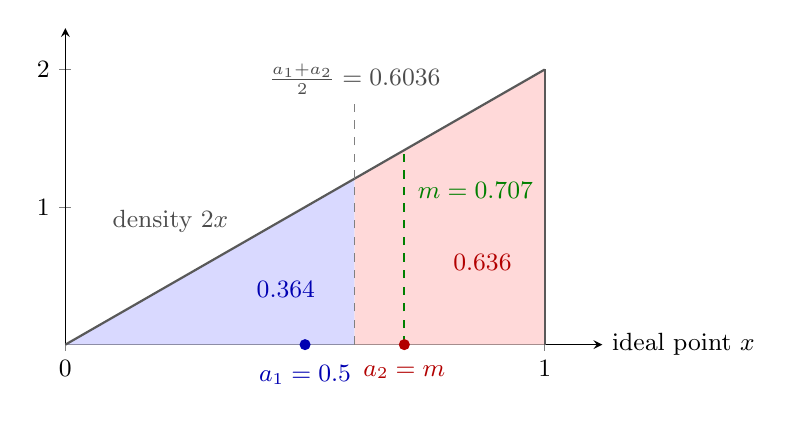
\begin{tikzpicture}[font=\small, >={Latex[length=2mm]}]
  \begin{axis}[
    axis lines=left, xmin=0, xmax=1.12, ymin=0, ymax=2.3,
    xtick={0,1}, ytick={1,2},
    xlabel={ideal point $x$},
    xlabel style={anchor=west, at={(axis description cs:1.0,0.0)}},
    width=8.4cm, height=5.6cm, clip=false]
    % vote shares under the density
    \addplot[draw=none, fill=blue!15, domain=0:0.6036, samples=2] {2*x} \closedcycle;
    \addplot[draw=none, fill=red!15, domain=0.6036:1, samples=2] {2*x} \closedcycle;
    \addplot[gray!70!black, thick, domain=0:1, samples=2] {2*x};
    \draw[gray!70!black, thick] (axis cs:1,0) -- (axis cs:1,2);
    \node[gray!60!black, anchor=east] at (axis cs:0.36,0.9) {density $2x$};
    % midpoint between the platforms
    \draw[gray, dashed, thin] (axis cs:0.6036,0) -- (axis cs:0.6036,1.75);
    \node[gray!60!black, anchor=south] at (axis cs:0.6036,1.75) {$\tfrac{a_1+a_2}{2}=0.6036$};
    % median
    \draw[green!50!black, thick, dashed] (axis cs:0.7071,0) -- (axis cs:0.7071,1.414);
    % shares
    \node[blue!70!black] at (axis cs:0.46,0.4) {$0.364$};
    \node[red!70!black] at (axis cs:0.87,0.6) {$0.636$};
    % platforms
    \fill[blue!70!black] (axis cs:0.5,0) circle (2pt);
    \node[blue!70!black, anchor=north] at (axis cs:0.5,-0.08) {$a_1=0.5$};
    \fill[red!70!black] (axis cs:0.7071,0) circle (2pt);
    \node[red!70!black, anchor=north] at (axis cs:0.7071,-0.08) {$a_2=m$};
    \node[green!50!black, anchor=west] at (axis cs:0.715,1.12) {$m=0.707$};
  \end{axis}
\end{tikzpicture}
\end{document}
